\documentclass{article}
\usepackage{graphicx}
\usepackage{booktabs}
\usepackage{geometry}
\usepackage{float}
\usepackage{listings}
\usepackage{xcolor}
\usepackage{subcaption}
\usepackage{setspace}
\usepackage[slantfont,boldfont]{xeCJK}
\usepackage{fontspec}

% 字体设置（存在即用，缺失则回退）


\geometry{a4paper,scale=0.8}
\onehalfspacing

\definecolor{dkgreen}{rgb}{0,0.6,0}
\definecolor{gray}{rgb}{0.5,0.5,0.5}
\definecolor{mauve}{rgb}{0.58,0,0.82}
\lstset{
frame=tb,
language=Python,
aboveskip=3mm,
belowskip=3mm,
showstringspaces=false,
columns=flexible,
basicstyle={\small\ttfamily},
numbers=left,
numberstyle=\tiny\color{gray},
keywordstyle=\color{blue},
commentstyle=\color{dkgreen},
stringstyle=\color{mauve},
breaklines=true,
breakatwhitespace=true,
tabsize=2
}

\newcommand{\tbplaceholder}[2][0.92\linewidth]{%
\fbox{\parbox[c][0.28\textheight][c]{#1}{\centering\small #2}}%
}

\title{实验二\hspace{2em}实验报告}
\author{人工智能2402\hspace{1em}陈子硕}
\date{\today}

\begin{document}

\maketitle

\section{实验环境说明}
本实验围绕“定制新的张量运算”展开，核心任务是分别使用 Python API 与 C++ 扩展实现自定义算子，并在 MNIST 任务上比较其训练可用性与性能表现。

\begin{table}[H]
\centering
\caption{实验硬件环境}
\label{tab:hardware_env}
\begin{tabular}{p{0.28\linewidth} p{0.64\linewidth}}
\toprule
项目 & 配置 \\
\midrule
CPU & Intel(R) Xeon(R) Gold 6226R CPU @ 2.90GHz \\
CPU 拓扑 & 双路，16 cores/socket，2 threads/core，共 64 逻辑 CPU \\
系统内存 & 251 GiB \\
GPU & NVIDIA GeForce RTX 3090 $\times 8$ \\
单卡显存 & 24576 MiB（24 GiB） \\
训练方式 & 单卡训练，未启用多卡并行 \\
NVIDIA Driver & 570.133.20 \\
\bottomrule
\end{tabular}
\end{table}

\begin{table}[H]
\centering
\caption{实验软件环境}
\label{tab:software_env}
\begin{tabular}{p{0.28\linewidth} p{0.64\linewidth}}
\toprule
项目 & 配置 \\
\midrule
操作系统 & Ubuntu 20.04.6 LTS，Linux 5.15.0-139-generic \\
Python & 3.10.19（\texttt{conda} 环境 \texttt{ai\_lab}） \\
PyTorch & 2.6.0+cu124 \\
CUDA & PyTorch CUDA 12.4；\texttt{nvidia-smi} 显示 12.8；\texttt{nvcc} 12.1.105 \\
编译器 & GCC/G++ 9.4.0 \\
工具链 & TensorBoard、\texttt{torch.profiler}、pybind11、torch cpp extension \\
\bottomrule
\end{tabular}
\end{table}

\section{实验目标与实验设计}
根据指导书要求，本实验需要完成以下五项工作：
\begin{enumerate}
    \item 基于 Python API 实现自定义 Linear 张量运算；
    \item 基于 C++ API 实现自定义 Linear 张量运算；
    \item 基于 Python API 设计并实现新的张量算子 Bent Identity；
    \item 基于 C++ API 实现同一自定义张量算子；
    \item 对内置算子、Python 自定义算子、C++ 自定义算子进行统一口径下的性能比较。
\end{enumerate}

\begin{table}[H]
\centering
\caption{实验脚本与实现矩阵}
\label{tab:script_matrix}
\begin{tabular}{p{0.24\linewidth} p{0.13\linewidth} p{0.20\linewidth} p{0.18\linewidth} p{0.12\linewidth}}
\toprule
脚本 / 简称 & 平台 & Linear & Activation & 角色 \\
\midrule
\texttt{mnist\_basic.py} / \texttt{B-bias} & 内置 & \texttt{nn.Linear(bias=True)} & \texttt{ReLU} & 主线 \\
\texttt{mnist\_custom\_linear.py} / \texttt{P-L} & Python & 自定义 Linear & \texttt{ReLU} & 主线 \\
\texttt{mnist\_custom\_linear\_cpp.py} / \texttt{C-L} & C++ & 自定义 C++ Linear & \texttt{ReLU} & 主线 \\
\texttt{mnist\_custom\_linear+op.py} / \texttt{P-L+BI} & Python & 自定义 Linear & Bent Identity & 主线 \\
\texttt{mnist\_custom\_linear+op\_cpp.py} / \texttt{C-L+BI} & C++ & 自定义 C++ Linear & C++ Bent Identity & 主线 \\
\texttt{mnist\_basic\_nobias.py} / \texttt{B-nobias} & 内置 & \texttt{nn.Linear(bias=False)} & \texttt{ReLU} & 补充 \\
\texttt{mnist\_custom\_linear\_cuda.py} / \texttt{CUDA-L} & CUDA & 自定义 CUDA Linear & \texttt{ReLU} & 补充 \\
\texttt{mnist\_custom\_linear\_cuda\_nobias} / \texttt{CUDA-L-NoBias} & CUDA & CUDA Linear(NoBias) & \texttt{ReLU} & 补充 \\
\bottomrule
\end{tabular}
\end{table}


\section{关键实现过程}
\subsection{阶段一：Python API 实现自定义 Linear}
在 \texttt{my\_linear.py} 中，通过继承 \texttt{torch.autograd.Function} 手写 Linear 的前向与反向传播。为突出算子原理，这里展示核心的无 bias 形式：
\[
Y = XW^T,\qquad
\frac{\partial L}{\partial X} = \frac{\partial L}{\partial Y}W,\qquad
\frac{\partial L}{\partial W} = \left(\frac{\partial L}{\partial Y}\right)^T X
\]

\begin{lstlisting}[language=Python,caption={\texttt{my\_linear.py} 中自定义 Linear 的前向与反向},label={lst:py_linear_impl}]
class MylinearFuct(torch.autograd.Function):
    @staticmethod
    def forward(ctx: FunctionCtx, input: torch.Tensor, weight: torch.Tensor):
        ctx.save_for_backward(input, weight)
        return input.mm(weight.t())

    @staticmethod
    def backward(ctx: FunctionCtx, *grad_outputs):
        grad_output = grad_outputs[0]
        input, weight = ctx.saved_tensors
        grad_input = grad_output.mm(weight) if ctx.needs_input_grad[0] else None
        grad_weight = grad_output.t().mm(input) if ctx.needs_input_grad[1] else None
        return grad_input, grad_weight
\end{lstlisting}

\subsection{阶段二：C++ API 实现自定义 Linear}
在 \texttt{mylinear\_cpp\_extension/mylinear.cpp} 中实现 C++ 版本的 \texttt{forward/backward}，再通过 \texttt{setup.py} 编译为可在 Python 侧导入的扩展模块。训练脚本中仍需使用 \texttt{autograd.Function} 进行封装，以便与计算图对接。

\begin{lstlisting}[language=C++,caption={\texttt{mylinear.cpp} 中 Linear 算子核心实现},label={lst:cpp_linear_impl}]
std::vector<torch::Tensor> mylinear_forward(
    torch::Tensor input,
    torch::Tensor weights) {
    auto output = torch::mm(input, weights.transpose(0, 1));
    return {output};
}

std::vector<torch::Tensor> mylinear_backward(
    torch::Tensor grad_output,
    torch::Tensor input,
    torch::Tensor weights) {
    auto grad_input = torch::mm(grad_output, weights);
    auto grad_weights = torch::mm(grad_output.transpose(0, 1), input);
    return {grad_input, grad_weights};
}
\end{lstlisting}

\begin{lstlisting}[language=Python,caption={\texttt{mylinear\_cpp\_extension/setup.py} 构建入口},label={lst:cpp_linear_setup}]
from setuptools import setup
from torch.utils import cpp_extension

setup(
    name='mylinear_cpp',
    ext_modules=[cpp_extension.CppExtension('mylinear_cpp', ['mylinear.cpp'])],
    cmdclass={'build_ext': cpp_extension.BuildExtension}
)
\end{lstlisting}

\subsection{阶段三：Python API 实现自定义张量运算}
本实验选择 Bent Identity 作为新的激活函数，其前向表达式与导数为：
\[
f(x)=x+\frac{\sqrt{x^2+1}-1}{2},\qquad
f'(x)=1+\frac{x}{2\sqrt{x^2+1}}
\]
该算子只依赖基础张量运算，导数连续、数值行为平滑，适合用于观察“算子复杂度变化”对训练与性能的影响。

\begin{lstlisting}[language=Python,caption={\texttt{my\_op.py} 中 Bent Identity 的前向与反向},label={lst:py_bent_impl}]
class BentIdentityFunc(torch.autograd.Function):
    @staticmethod
    def forward(ctx: FunctionCtx, myinput: torch.Tensor):
        ctx.save_for_backward(myinput)
        return myinput + (torch.sqrt(torch.square(myinput) + 1) - 1) / 2

    @staticmethod
    def backward(ctx: FunctionCtx, grad_out: torch.Tensor):
        (myinput,) = ctx.saved_tensors
        grad_x = 1 + myinput / (2 * torch.sqrt(torch.square(myinput) + 1))
        return grad_out * grad_x
\end{lstlisting}

\begin{figure}[H]
    \centering
    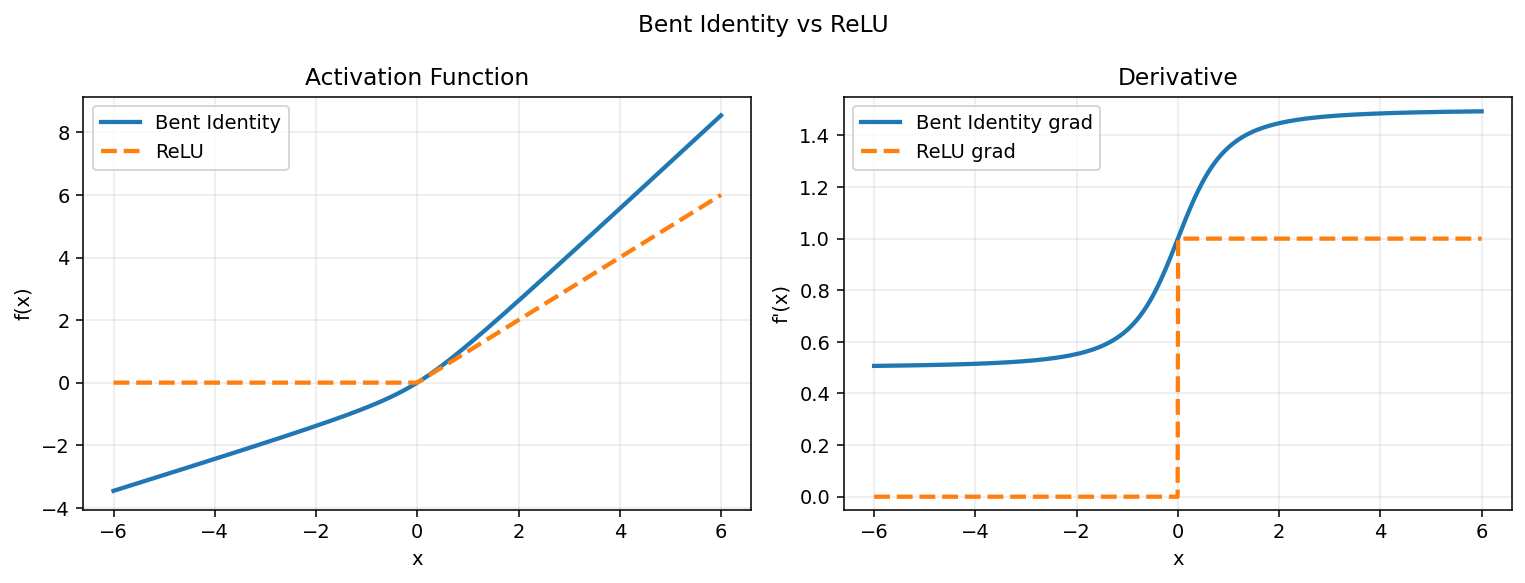
\includegraphics[width=0.96\linewidth]{figures/bent_identity_vs_relu.png}
    \caption{Bent Identity 与 ReLU 的函数形状对比。Bent Identity 更平滑，导数也连续。}
    \label{fig:bent_visual}
\end{figure}

\subsection{阶段四：C++ API 实现自定义张量运算}
在 \texttt{my\_cpp\_op/my\_op\_c++.cpp} 中实现 Bent Identity 的 C++ 版本，并通过扩展接口暴露 \texttt{forward} 与 \texttt{backward}。Python 训练脚本再将其封装为可参与自动求导的模块。

\begin{lstlisting}[language=C++,caption={\texttt{my\_op\_c++.cpp} 中 Bent Identity 算子实现},label={lst:cpp_bent_impl}]
torch::Tensor BentForward(torch::Tensor input) {
    return input + (torch::sqrt(input * input + 1) - 1) / 2;
}

torch::Tensor BentBackward(torch::Tensor grad_out, torch::Tensor input) {
    auto grad_x = 1 + input / (2 * torch::sqrt(input * input + 1));
    return grad_out * grad_x;
}
\end{lstlisting}

\subsection{Python 与 C++ 结构差异}
Python 版与 C++ 版的数学公式完全一致，差异主要体现在接口边界：
\begin{itemize}
    \item Python 版直接在 \texttt{torch.autograd.Function} 中定义前后向，开发调试成本较低；
    \item C++ 版需要先在扩展中导出接口，再由 Python 侧包装进 \texttt{autograd}；
    \item 当前 C++ Linear 的核心仍调用 ATen 的矩阵乘，并非 fused CUDA kernel，因此性能提升不一定显著；
    \item C++ 扩展构建、加载和 Python 边界调用本身也会带来额外工程开销。
\end{itemize}

\section{统一实验配置与观测口径}
\subsection{统一训练参数}
当前长程对比统一采用以下配置：
\begin{itemize}
    \item 数据集：MNIST；
    \item \texttt{batch\_size=64}，\texttt{test\_batch\_size=1000}；
    \item \texttt{epochs=14}；
    \item 优化器为 Adadelta，学习率 \texttt{lr=1.0}；
    \item 学习率调度为 \texttt{StepLR(gamma=0.7)}；
    \item \texttt{seed=1}，\texttt{log\_interval=10}；
    \item 单卡训练，不启用 \texttt{DataParallel}。
\end{itemize}

\subsection{日志与性能观测}
各脚本统一记录以下 TensorBoard 标量：
\begin{itemize}
    \item 训练损失：\texttt{train/loss\_epoch}；
    \item 测试精度：\texttt{test/accuracy}。
\end{itemize}

Profiler 调度统一为：
\[
\texttt{wait=20,\ warmup=20,\ active=30,\ repeat=1}
\]
trace 输出到 \texttt{runs/<exp\_name>/profiler\_traces/}。由于当前日志中没有稳定的 \texttt{perf/time\_to\_99\_sec} 秒级指标，本文在收敛速度对比时以“达到 99\% 精度所需 epoch（\texttt{epoch\_to\_99}）”作为替代口径。

\section{实验结果与分析}
\subsection{训练可用性验证}
5 组主线实验都能够完整训练到结束，未出现梯度爆炸、\texttt{NaN} 或反向传播中断。这说明 Python 版和 C++ 版的自定义 Linear 与 Bent Identity 都已经正确接入自动求导图，具备工程可用性。
结合 TensorBoard 标量可见，\texttt{B-bias}、\texttt{P-L} 与 \texttt{C-L} 的训练损失都能随 epoch 稳定下降并收敛到 0.03--0.04 区间，说明数值稳定性较好；两组 Bent Identity 版本的损失下降更慢，最终停留在约 0.044 附近，这也与其测试精度略低的现象一致。

\subsection{主线实验结果（14 epoch）}
表~\ref{tab:perf_compare_main} 汇总了 5 组主线实验的关键结果。

\begin{table}[H]
\centering
\caption{主线实验结果对比（14 epoch）}
\label{tab:perf_compare_main}
\begin{tabular}{p{0.14\linewidth} p{0.12\linewidth} p{0.14\linewidth} p{0.11\linewidth} p{0.11\linewidth} p{0.13\linewidth}}
\toprule
代号 & 最终 Train Loss & 最优 Test Acc(\%) & 最优 Epoch & 到 99\% Epoch & 平均 Step(ms) \\
\midrule
\texttt{B-bias} & 0.029209 & 99.17 & 10 & 5 & 9.407 \\
\texttt{P-L} & 0.038230 & 99.10 & 9 & 5 & 9.044 \\
\texttt{C-L} & 0.038015 & 99.11 & 11 & 6 & 9.508 \\
\texttt{P-L+BI} & 0.043276 & 98.70 & 11 & 未达到 & 11.206 \\
\texttt{C-L+BI} & 0.044140 & 98.71 & 13 & 未达到 & 10.848 \\
\bottomrule
\end{tabular}
\end{table}

\begin{figure}[H]
    \centering
    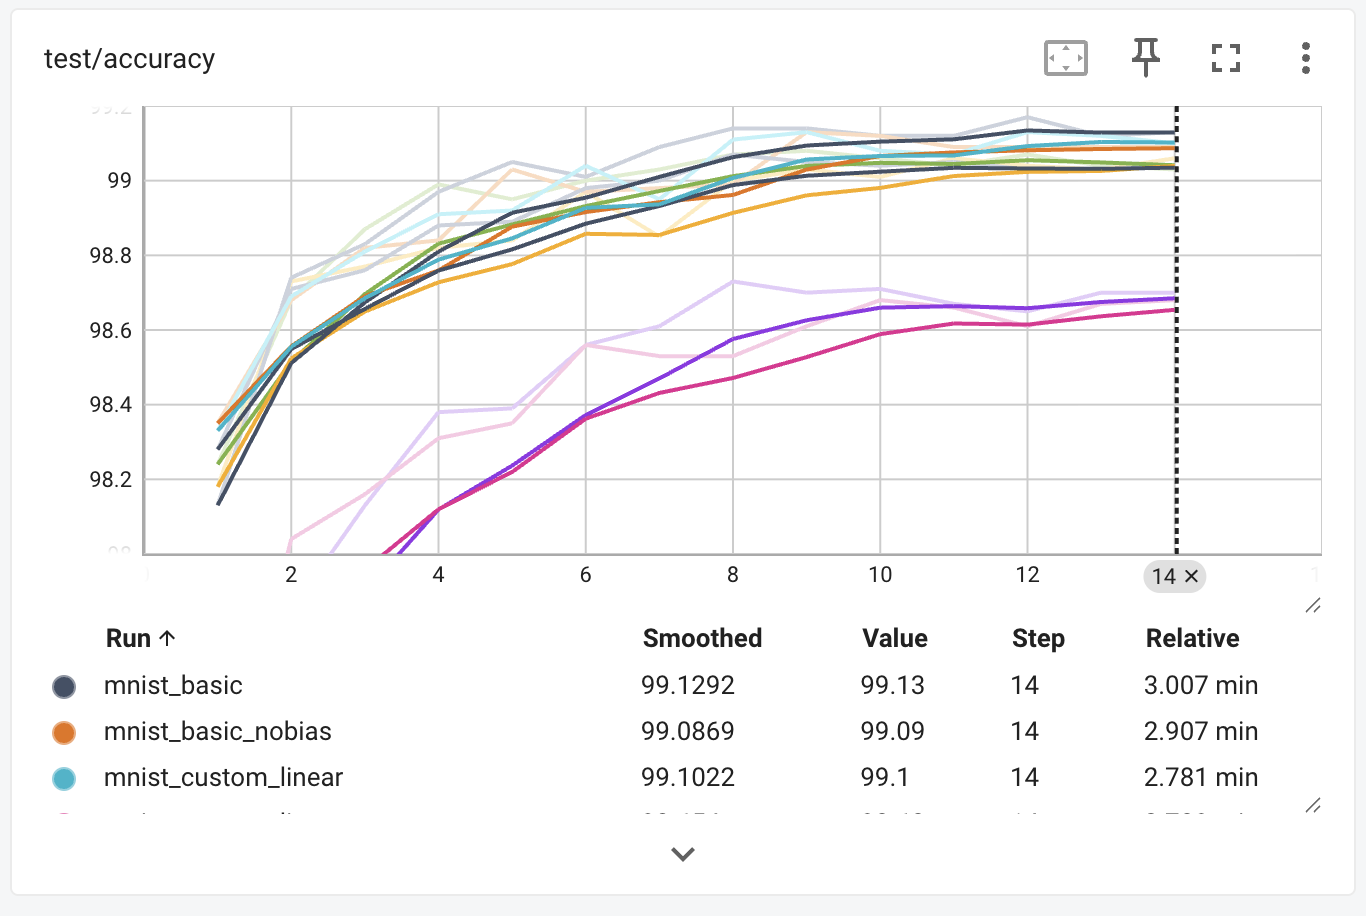
\includegraphics[width=0.96\linewidth]{figures/testandacc.png}
    \caption{不同实现方式的 \texttt{test/accuracy} 曲线截图。主线 Linear 组都能稳定逼近 99\%，而引入 Bent Identity 后准确率整体下移。}
    \label{fig:test_accuracy_all}
\end{figure}

从表中可以看出，主线 Linear 组（\texttt{B-bias}、\texttt{P-L}、\texttt{C-L}）都在 14 epoch 内达到或逼近 99\% 的测试精度，说明内置、Python 自定义与 C++ 扩展三类实现的数学逻辑都成立。就主线组而言，\texttt{P-L} 的平均 step 时间最低，\texttt{C-L} 略慢于它，但差距很小；因此“迁移到 C++”并不会自动带来明显加速。

引入 Bent Identity 后，\texttt{P-L+BI} 与 \texttt{C-L+BI} 在 14 epoch 内均未达到 99\%，最终精度也低于 ReLU 版本，同时平均 step 时间上升到 10.8--11.2 ms 区间。这说明本实验中更显著的影响因素不是实现语言，而是算子本身的复杂度。

\subsection{补充实验：bias 与 CUDA 的影响}
为进一步说明 bias 与 CUDA 对结果的影响，本文还参考了 \texttt{B-nobias}、\texttt{CUDA-L} 与 \texttt{CUDA-L-NoBias} 三组补充实验。它们的意义在于说明：性能结论不仅受“Python / C++ / CUDA”平台影响，也受“是否包含 bias”这一实现口径影响。考虑到指导书前两阶段以不带偏置项的 Linear 为例，严格讨论平台差异时，也应把 \texttt{B-nobias} 作为辅助参考。

补充统计显示，在无 bias 口径下，\texttt{mnist\_custom\_linear\_cuda\_nobias} 的平均 step 时间可进一步降到 9.421 ms，低于含 bias 的内置基线与主线 C++ 版本。

\begin{figure}[H]
    \centering
    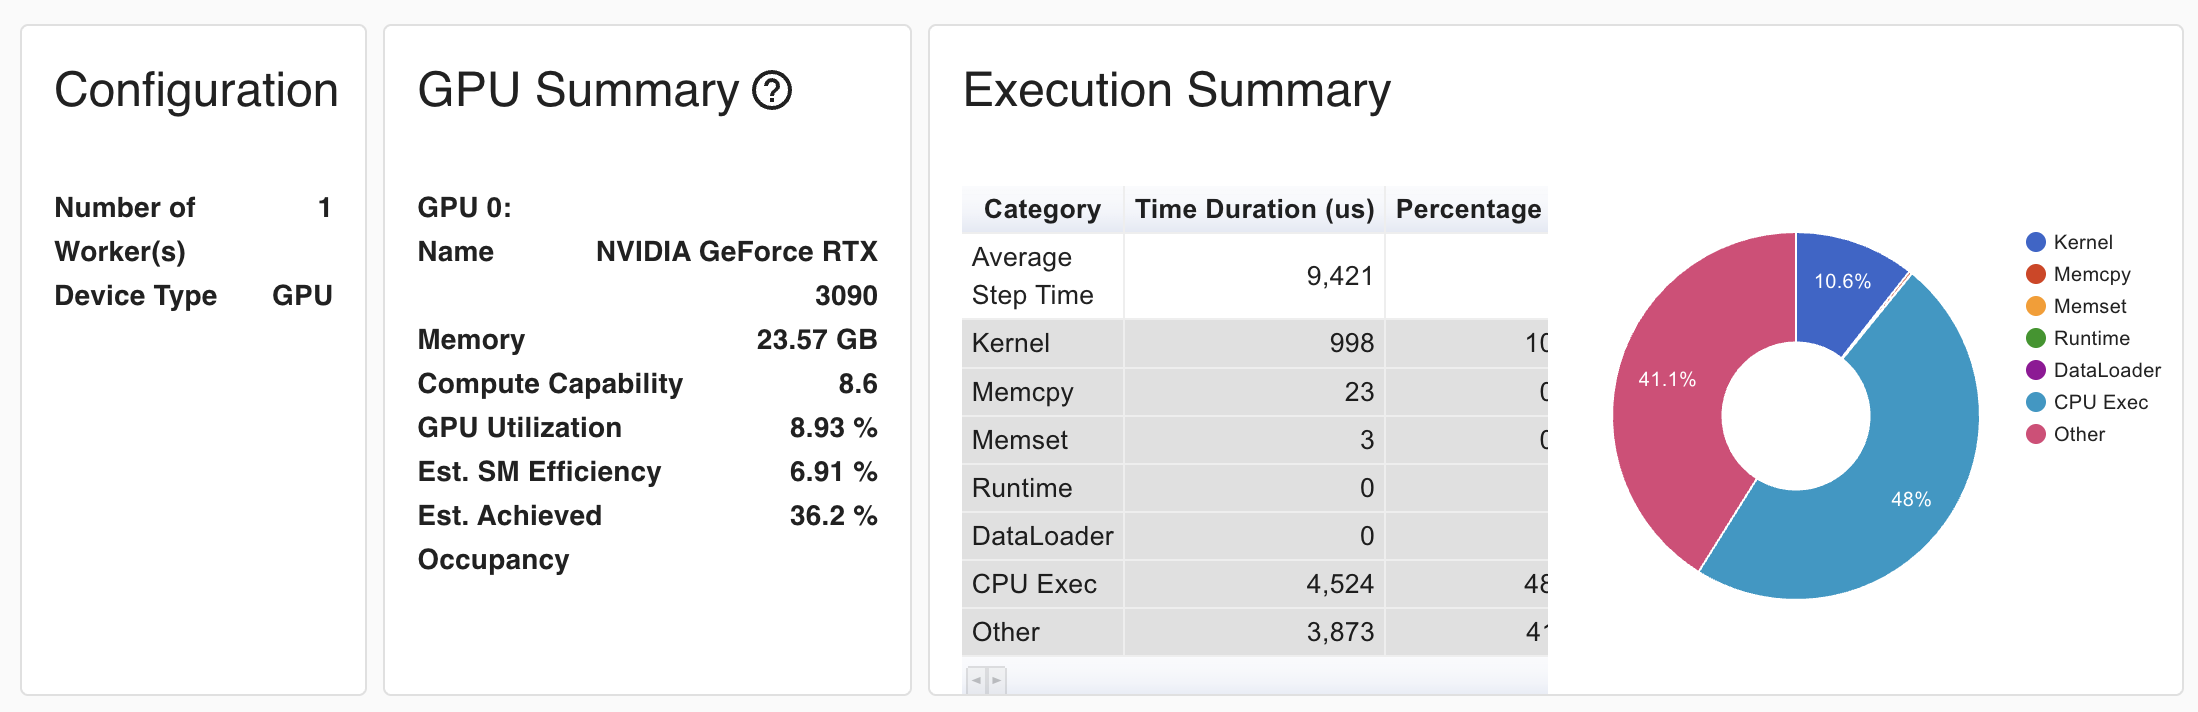
\includegraphics[width=0.96\linewidth]{figures/CUDATime.png}
    \caption{\texttt{CUDA-L-NoBias} 的 Profile 摘要截图。可以看到当前实验为单卡 GPU 训练，平均 step 时间约为 9.421 ms，同时 CPU Exec 与 Other 仍占较大比例。}
    \label{fig:cuda_profile_summary}
\end{figure}

\subsection{Profiler 热点解读}
\begin{figure}[H]
    \centering
    \begin{subfigure}[t]{0.48\linewidth}
        \centering
        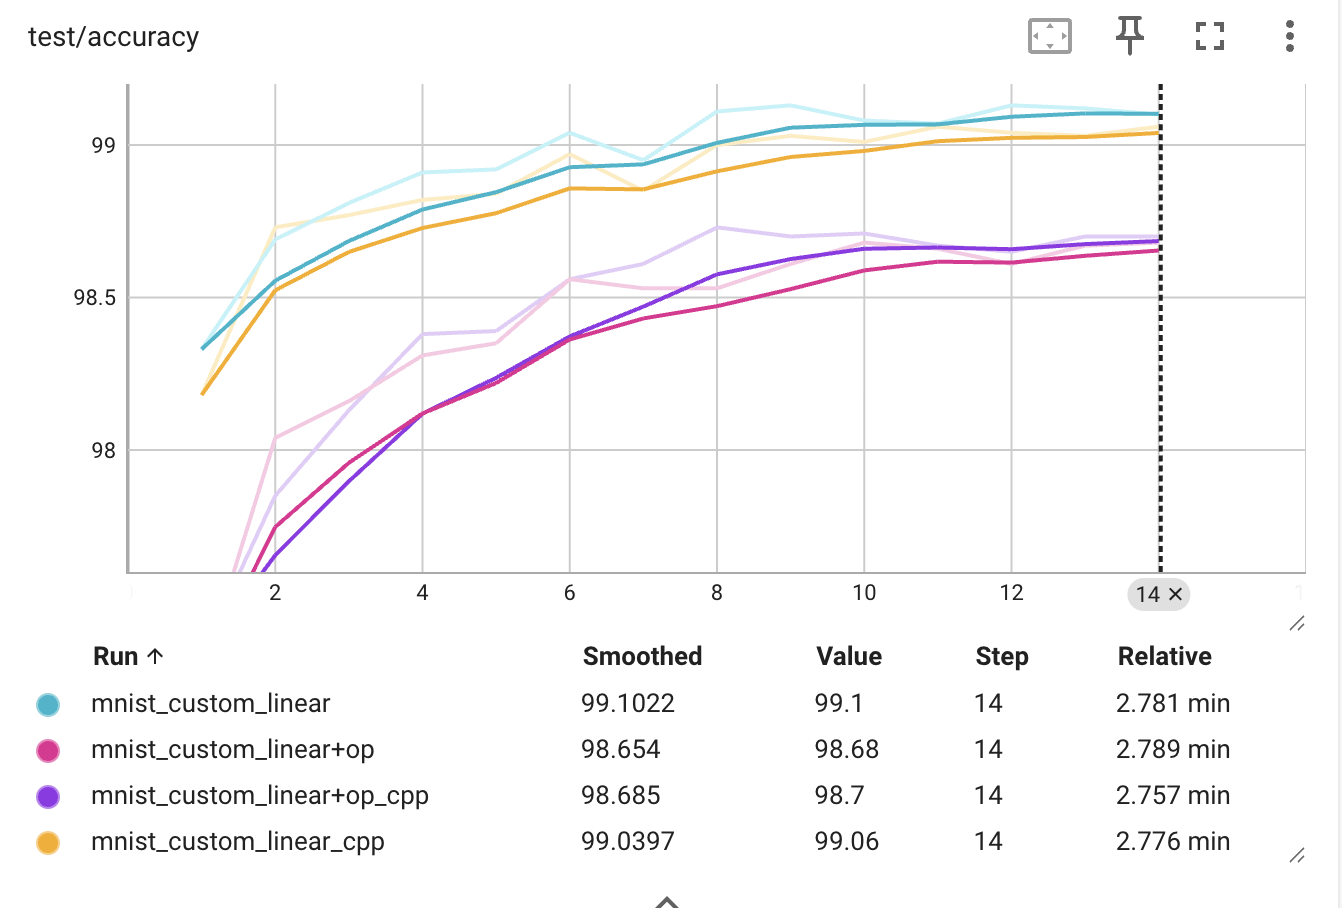
\includegraphics[width=\linewidth]{figures/optestacc.png}
        \caption{自定义算子组的 \texttt{test/accuracy} 曲线}
    \end{subfigure}
    \hfill
    \begin{subfigure}[t]{0.48\linewidth}
        \centering
        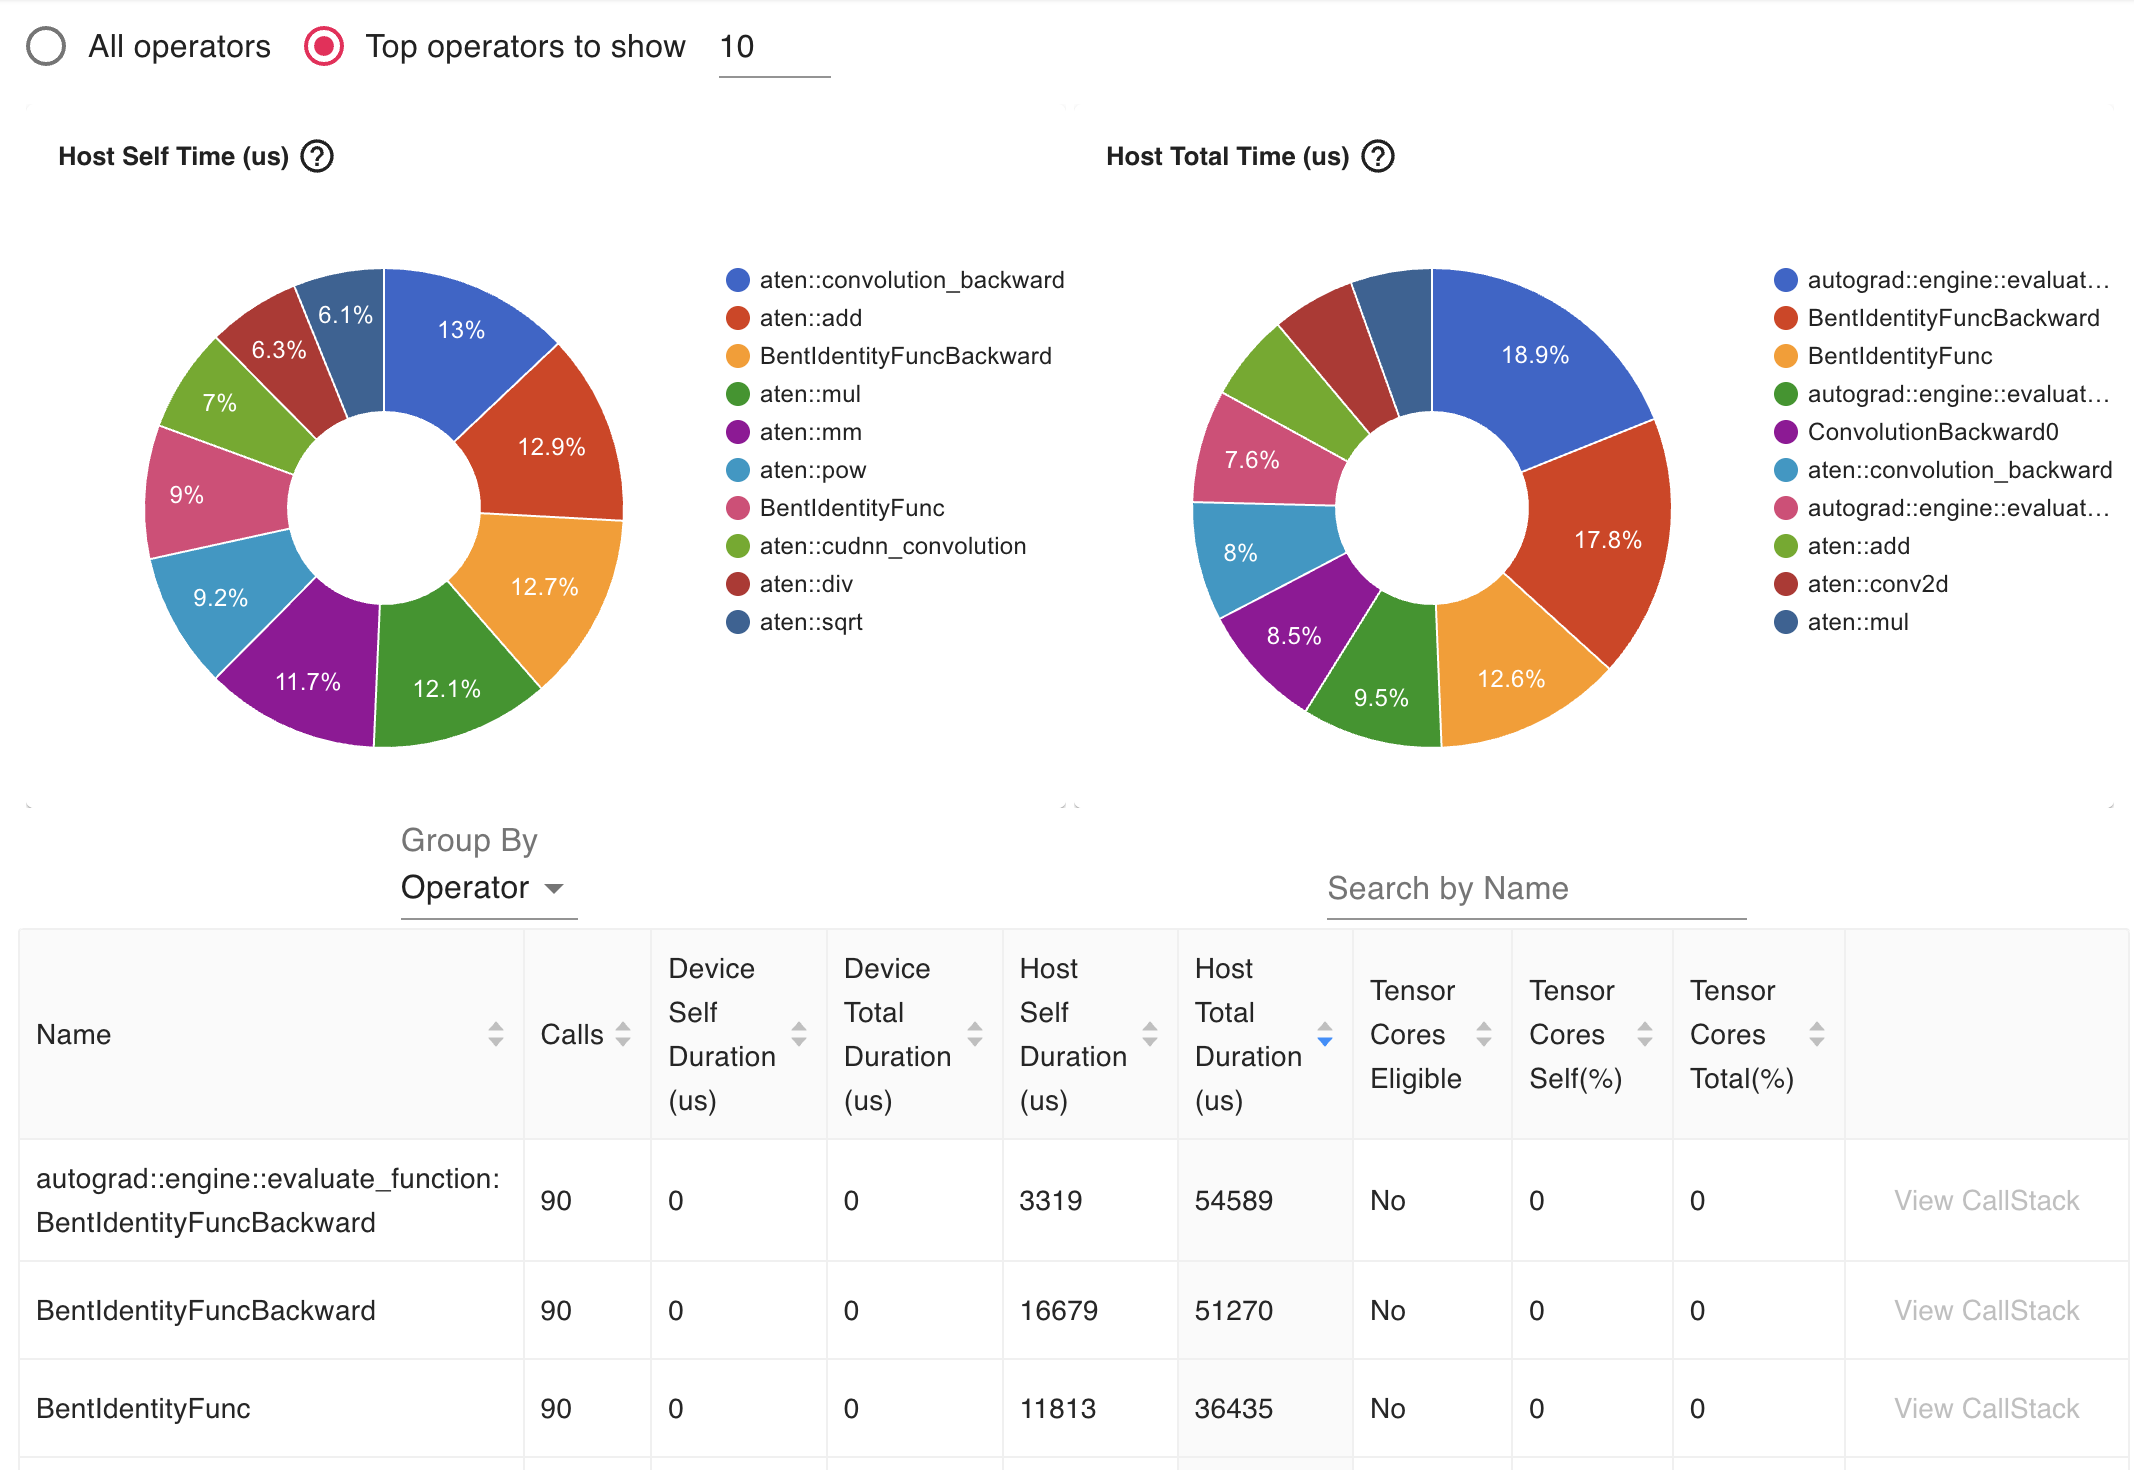
\includegraphics[width=\linewidth]{figures/BiTime.png}
        \caption{Bent Identity 组的热点算子截图}
    \end{subfigure}
    \caption{Bent Identity 对收敛和热点分布的影响}
    \label{fig:bi_accuracy_and_hotspots}
\end{figure}

可以得到以下观察：
\begin{itemize}
    \item \texttt{mnist\_basic}、\texttt{mnist\_custom\_linear}、\texttt{mnist\_custom\_linear\_cpp} 的热点主要集中在卷积反向相关路径，如 \texttt{ConvolutionBackward0}；
    \item 在 \texttt{mnist\_custom\_linear+op} 与 \texttt{mnist\_custom\_linear+op\_cpp} 中，\texttt{BentIdentity} 的前后向成为显著热点，说明额外激活逻辑引入了稳定的开销；
    \item CPU operator 统计中，“Top3 之外的 Other 占比”约为 74\%--84\%，表明时间分散在大量小算子和框架开销中，这在 MNIST 小模型场景里是常见现象。
\end{itemize}

因此，本实验更适合把 Profiler 用于“定位为什么慢”，而不是直接把带 profiler 的 step 时间当作最终速度排名的唯一依据。

\section{实验中的问题与修复}
本次实验中遇到的问题主要包括：
\begin{itemize}
    \item 预处理口径不一致：早期调试阶段，不同脚本在归一化与输入处理上存在差异，导致精度对比失真；统一后结果才具备可比性；
    \item Profiler 对小模型干扰明显：MNIST 网络本身较小，开启 profiler 后固定开销占比会被放大，因此分析时需要区分“真实训练开销”和“观测工具开销”；
    \item 扩展构建路径错误：出现 \texttt{missing and no known rule to make it} 时，需要切换到扩展源码目录再执行 \texttt{setup.py}；
    \item 数据目录权限问题：MNIST 数据写入到不可写目录会触发 \texttt{Permission denied}，统一使用项目内可写目录即可解决。
\end{itemize}

\section{实验总结}
本实验完成了从 Python 到 C++ 的自定义算子实现链路，并在 MNIST 任务上验证了其训练可用性。结果表明，主线 Linear 组在精度上都能逼近同一区间，Python 自定义 Linear 与 C++ 扩展版的差距并不大；如果没有进一步做 kernel 融合或减少边界开销，C++ 扩展并不会天然显著快于 Python 版。

另一方面，Bent Identity 的影响更直接也更稳定：它带来了额外的前后向计算成本，使平均 step 时间明显上升，同时最终精度略低于对应的 ReLU 版本。补充实验还说明，bias 口径会显著影响性能结论，因此在解释“哪个实现更快”时，必须把算子复杂度、是否带 bias、Profiler 干扰和任务规模一起考虑，而不能只看实现语言。

综合来看，本实验可以得到以下结论：
\begin{enumerate}
    \item 自定义 Linear 与 Bent Identity 都能够正确接入 \texttt{autograd} 并完成训练；
    \item 在 MNIST 上，最终精度差异有限，平均 step 时间与 Profiler 热点更能体现实现差异；
    \item C++ 扩展不等于自动加速，算子复杂度和实验口径往往比“实现语言”更能决定结果；
    \item 若目标是进一步提速，后续应优先考虑 kernel 级优化、算子融合以及无 profiler 的纯基准测试。
\end{enumerate}
\end{document}
